\chapter{Discussion}
Please tell more about conclusion and how to the next work of this study.

\section{Imron Sumadireja / 1164076}
\subsection{Teori}
\begin{enumerate}

\item Jelaskan kenapa file suara harus di lakukan MFCC. Dilengkapi dengan ilustrasi atau gambar. \par
MFCC merupakan koefisien yang merepresentasikan audio. Ekstraksi ciri dalam proses ini ditandai dengan pengubahan data suara menjadi citra berupa spektrum gelombang. File audio dilakukan MFCC itu agar objek suara dapat diubah menjadi bentuk matrix. Suara tersebut akan menjadi vektor yang nantinya akan diolah sebagai keluaran. Untuk ilustrasi sederhananya bisa dilihat pada gambar \ref{cc1}. Gambar tersebut menjelaskan tahapan-tahapan kenapa file suara harus dilakukan MFCC. Selain itu untuk memberikan kemudahan kepada mesin dalam mempelajari suara tersebut karena mesin tidak dapat membaca teks maka dari itu diperlukan MFCC untuk merubah suara tersebut menjadi vektor.
		\begin{figure}[!htbp]
		\centerline{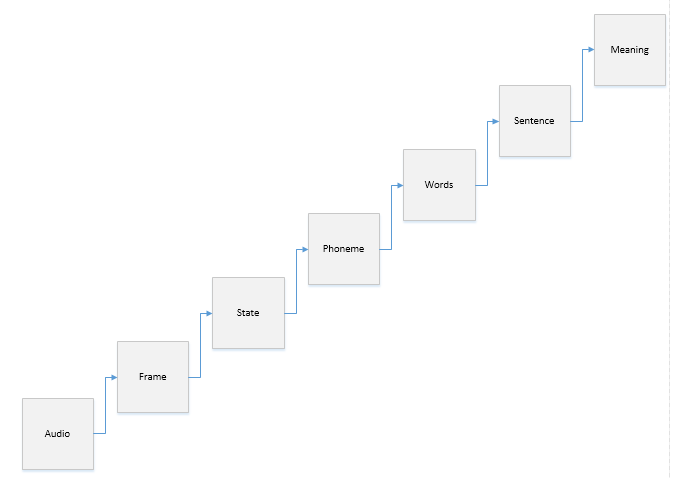
\includegraphics[width=0.5\textwidth]{figures/im/cc1.png}}
		\caption{MFCC.}
		\label{cc1}
		\end{figure}

\item Jelaskan konsep dasar neural network. Dilengkapi dengan ilustrasi atau gambar. \par
Konsep sederhana dari neural network hampir mirip dengan proses belajar pada anak-anak yakni dengan memetakan pola baru yang didapatkan dari inputan untuk membuat pola baru pada keluaran. Contoh sederhana tersebut menganalogikan kinerja otak manusia. Neural network itu sendiri terdiri dari sebuah unit pemroses yang disebut neuron yang berisi adder dan fungsi aktivasi. Fungsi aktivasi itu sendiri untuk mengatur keluaran yang diberikan oleh neuron. Neural network ini mengadopsi mekanisme berpikir sebuah sistem atau aplikasi yang menyerupai otak manusia, baik untuk pemrosesan berbagai sinyal elemen yang diterima, toleransi terhadap kesalahan/error, dan juga prallel processing. Karakteristik dari neural network dilihat dari pola hubungan antar neuron, metode penentuan bobot dari tiap koneksi, dan fungsi aktivasinya. Untuk ilustrasinya bisa dilihat pada gambar \ref{cc2}
		\begin{figure}[!htbp]
		\centerline{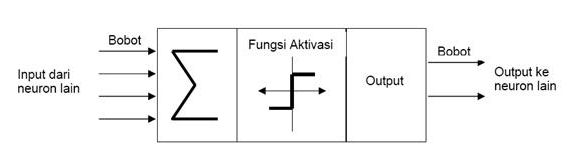
\includegraphics[width=0.5\textwidth]{figures/im/cc2.png}}
		\caption{Konsep Dasar Neural Network.}
		\label{cc2}
		\end{figure}

\item Jelaskan konsep pembobotan dalam neural network. Dilengkapi dengan ilustrasi atau gambar. \par
Pembobotan ini akan menentukan serta penanda dari sebuah konektivitas. Pada proses neural network dimulai dari input yang diterima oleh neuron beserta dengan nilai bobot dari tiap-tiap input yang ada. Setelah masuk ke dalam neuron, nilai input yang ada akan dijumlahkan oleh suatu fungsi penambahan. Hasil penjumlahan tersebut akan diproses oleh fungsi aktivasi oleh setiap neuron, hasil penjumlahan tersebut akan dibandingkan dengan nilai ambang tertentu. Jika nilai dari hasil penjumlahan tersebut melebihi nilai ambang maka aktivasi neuron akan dibatalkan, namun sebaliknya jika hasil penjumlahan dibawah nilai ambang maka neuron akan diaktifkan. Setelah neuron aktif selanjutnya akan mengirimkan nilai output melalui bobot-bobot keluarannya ke semua neuroon yang berhubungan. Ilustrasinya bisa dilihat pada gambar \ref{cc3}
		\begin{figure}[!htbp]
		\centerline{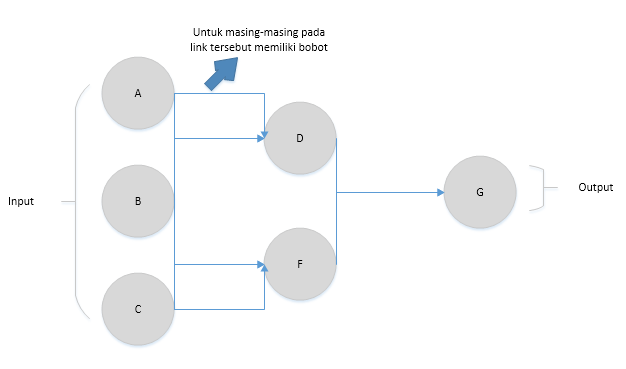
\includegraphics[width=0.5\textwidth]{figures/im/cc3.png}}
		\caption{Konsep Pembobotan Neural Network.}
		\label{cc3}
		\end{figure}

\item Jelaskan konsep fungsi aktifasi dalam neural network. Dilengkapi dengan ilustrasi atau gambar. \par
Fungsi aktivasi ini merupakan operasi matematik yang dikenakan pada sinyal output. Fungsi ini digunakan untuk mengaktifkan atau menonaktifkan neuron. Fungsi aktivasi ini terbagi setidaknya menjadi 6, dianranya sebagai berikut:
\begin{itemize}
\item a. Fungsi Undak Biner Hard Limit, fungsi ini biasanya digunakan oleh jaringan lapiran tunggal untuk mengkonversi nilai input dari suatu variabel yang bernilai kontinu ke suatu nilai output biner 0 atau 1.
\item b. Fungsi Undak Biner Threshold, fungsi ini menggunakan nilai ambang sebagai batasnya.
\item c. Fungsi Bipolar Symetric Hard Limit, fungsi ini memiliki output bernilai 1, 0 atau -1.
\item d. Fungsi Bipolar dengan Threshold, fungsi ini mempunyai output yang bernilai 1, 0 atau -1 untuk batas nilai ambang tertentu.
\item e. Fungsi Linear atau Identitas.
\end{itemize}
Untuk ilustrasi sederhananya bisa dilihat pada gambar \ref{cc4}. Gambar tersebut merupakan salah satu contoh dari fungsi aktivasi bipolar.
		\begin{figure}[!htbp]
		\centerline{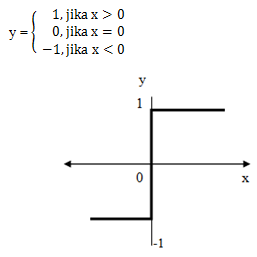
\includegraphics[width=0.5\textwidth]{figures/im/cc4.png}}
		\caption{Konsep Fungsi Aktivasi Neural Network.}
		\label{cc4}
		\end{figure}

\item Jelaskan cara membaca hasil plot dari MFCC. Dilengkapi dengan ilustrasi atau gambar. \par
Membaca plot MFCC ini bisa kita lihat pada gambar \ref{cc5}. Gambar tersebut menjelaskan bahwa pada waktu ke 5 daya atau desible yang dikelurakan pada nada tersebut paling keras pada 20 Hz, selain itu pada 40 -120 Hz itu daya atau desible yang dikeluarkan pada musik yang telah di plotting. Begitupun seterusnya bahwa warna yang paling gelap itu merupakan daya atau desible yang paling tinggi dibandingkan dengan warna yang cerah. Untuk yang berwarna merah itu suara dibawah pendengaran frekuensi manusia, jadi tidak dapat terdengar secara langsung. 
		\begin{figure}[!htbp]
		\centerline{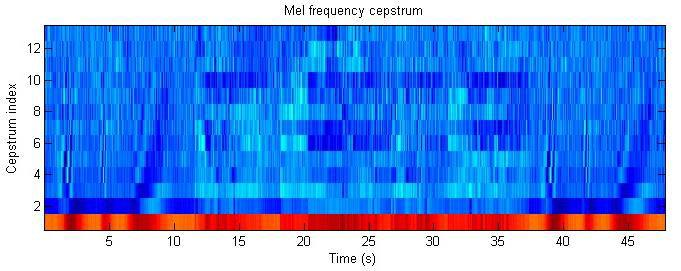
\includegraphics[width=0.5\textwidth]{figures/im/cc5.png}}
		\caption{Membaca Plot MFCC.}
		\label{cc5}
		\end{figure}

\item Jelaskan apa itu one-hot encoding. Dilengkapi dengan ilustrasi kode dan atau gambar. \par
Sederhananya one-hot encoding ini untuk merubah hasil data vektorisasi menjadi bilangan biner 0 dan 1 serta membuat keterangan pada atribut tersebut menjadi label. Unutuk ilustrasi sederhananya bisa dilihat pada gambar \ref{cc6}
		\begin{figure}[!htbp]
		\centerline{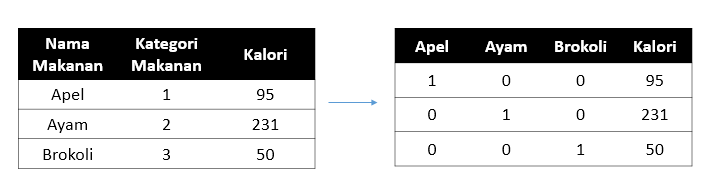
\includegraphics[width=0.5\textwidth]{figures/im/cc6.png}}
		\caption{One-Hot Encoding.}
		\label{cc6}
		\end{figure}

\item Jelaskan apa fungsi dari np.unique dan to categorical dalam kode program. Dilengkapi dengan ilustrasi atau gambar. \par
Fungsi dari np.unique adalah untuk menemukan elemen yang berbeda atau unik array, dan dapat mengembalikan elemen unik array tersebut yang diurutkan. Untuk ilustrasi sederhananya bisa dilihat pada gambar \ref{cc7}. Gambar tersebut menjelaskan bahwa unique itu sendiri akan mengambil data yang berbeda dari variabel a yang berada dalam fungsi array dan hasilnya seperti gambar tersebut.
		\begin{figure}[!htbp]
		\centerline{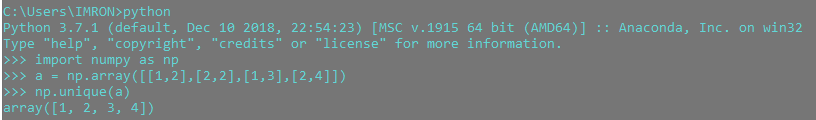
\includegraphics[width=0.5\textwidth]{figures/im/cc7.png}}
		\caption{np.unique.}
		\label{cc7}
		\end{figure}

Fungsi dari to\_categorical untuk mengubah vektor yang berupa integer menjadi matrix dengan kelas biner. Untuk ilustrasinya bisa dilihat pada gambar \ref{cc71}
		\begin{figure}[!htbp]
		\centerline{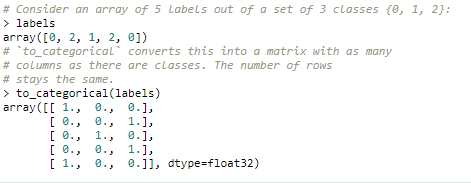
\includegraphics[width=0.5\textwidth]{figures/im/cc71.png}}
		\caption{to\_categorical.}
		\label{cc71}
		\end{figure}

\item Jelaskan apa fungsi dari Sequential dalam kode program. Dilengkapi dengan ilustrasi atau gambar.\par
Salah satu jenis model yang digunakan dalam perhitungan. Sequential ini membangun tumpukan linear yang berurutan. Contoh sederhananya sebagai berikut \ref{cc8}
		\begin{figure}[!htbp]
		\centerline{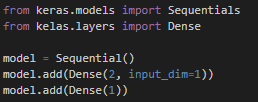
\includegraphics[width=0.5\textwidth]{figures/im/cc8.png}}
		\caption{Sequential.}
		\label{cc8}
		\end{figure}
\end{enumerate}

\subsection{Praktikum Program / Imron Sumadireja / 1164076}
\begin{enumerate}
\item Jelaskan isi dari data GTZAN Genre Collection dan data dari freesound. Buat kode program untuk meload data tersebut untuk digunakan pada MFCC. \par
Isi data dari GTZAN ini merupakan sekumpulan data yang berisi genre lagu yang di dalamnya terdapat 10 genre dengan masing-masing genre memiliki 100 lagu yang akan kita lakukan proses MFCC begitu pula dengan freesound yang membedakan hanya isi dari lagu tersebut, jika GTZAN memiliki beberapa genre kalau freesound hanya untuk 1 lagu saja. Untuk code programnya bisa dilihat seperti berikut: \lstinputlisting[firstline=16, lastline=25]{src/ron/Sounds.py} Baris pertama itu untuk me-load song yang akan kita gunakan, lalu pada baris keduanya akan membaca lagu tersebut dengan menggunakan librosa dan akan di lakukan vektorisasi dengan menggunakan MFCC. Setelah itu hasilnya akan di plot seperti gambar berikut \ref{classic1}
		\begin{figure}[!htbp]
		\centerline{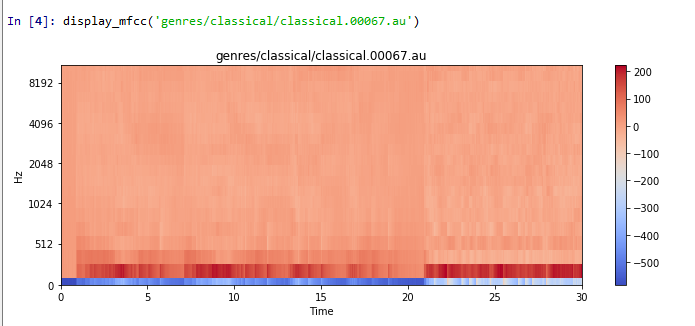
\includegraphics[width=0.5\textwidth]{figures/im/suara1.png}}
		\caption{Display MFCC.}
		\label{classic1}
		\end{figure}

\item Jelaskan perbaris kode program dengan kata-kata dan dilengkapi ilustrasi gambar fungsi dari display mfcc(). \par
 \lstinputlisting[firstline=27, lastline=27]{src/ron/Genre.py}
Code tersebut menjelaskan bahwa akan menampilkan hasil dari proses mfcc dan hasil yang akan ditampilkan dari code berikut seperti gambar \ref{suara2}
		\begin{figure}[!htbp]
		\centerline{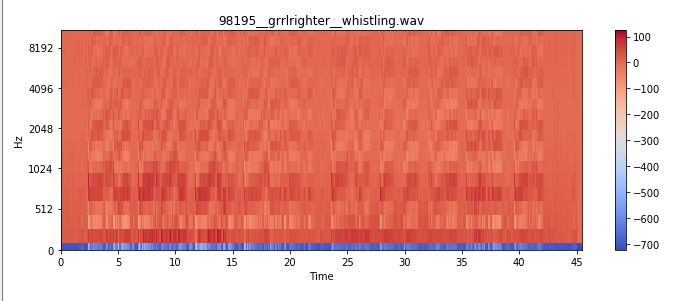
\includegraphics[width=0.5\textwidth]{figures/im/suara2.png}}
		\caption{Display MFCC.}
		\label{suara2}
		\end{figure}

\item Jelaskan perbaris kode program dengan kata-kata dan dilengkapi ilustrasi gambar fungsi dari extract features song(). \par
\lstinputlisting[firstline=46, lastline=54]{src/ron/Genre.py}
Baris pertama itu untuk me-load inputan. Pada baris kedua itu akan me-load data inputan dengan menggunakan librosa. Lalu selanjutnya untuk membuat sebuah fitur untuk mfcc dari y atau parameter inputan. Lalu akan me-return menjadi array dan akan mengambil 25000 data saja dari hasil vektorisasi dalam 1 lagu.  Hasil running dari code tersebut tidak mengeluarkan keluaran.

\item Jelaskan perbaris kode program dengan kata-kata dan dilengkapi ilustrasi gambar fungsi dari generate features and labels(). \par
\lstinputlisting[firstline=58, lastline=75]{src/ron/Genre.py}
Code tersebut akan melakukan fungsi yang sebelumnya kita telah jalankan. Lalu pada bagian genres itu disesuaikan dengan nama folder dataset. Untuk baris selanjutnya itu akan melakukan looping dari folder genres dengan ektensi .au. Lalu akan memanggil fungsi ekstrak lagu. Pada setiap file yang terdapat pada folder itu akan di ekstrak menjadi vektor dan akan dimasukan kedalam fitur. Dan fungsi append itu menumpuk file-file yang telah di vektorisasi. Hasil dari code tersebut tidak menampilkan keluaran.

\item Jelaskan dengan kata dan praktek kenapa penggunaan fungsi generate features and labels() sangat lama ketika meload dataset genre. \par
\lstinputlisting[firstline=78, lastline=78]{src/ron/Genre.py}
Karena mesin akan melakukan vektorisasi terhadap semua file yang berada pada setiap foldernya, di sini terdapat 10 folder dengan masing-masing folder terdiri atas 100 buah lagu, setiap lagu tersebut akan dilakukan vektorisasi atau ekstraksi data menggunakan mfcc. Makanya proses itu cukup memakan waktu. Hasilnya bisa dilihat pada gambar \ref{suara3} dan \ref{suara4}. Bedanya float 64 dengan 32 itu kapasitas variabelnya saja.
		\begin{figure}[!htbp]
		\centerline{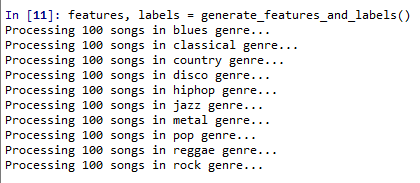
\includegraphics[width=0.5\textwidth]{figures/im/suara3.png}}
		\caption{Load Data.}
		\label{suara3}
		\end{figure}

		\begin{figure}[!htbp]
		\centerline{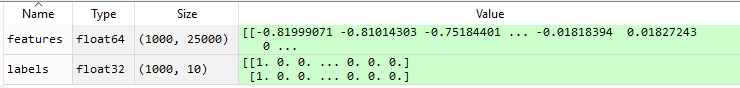
\includegraphics[width=0.5\textwidth]{figures/im/suara4.png}}
		\caption{Hasil Load Data.}
		\label{suara4}
		\end{figure}

\item Jelaskan kenapa harus dilakukan pemisahan data training dan data set sebesar 80 persen? \par
\lstinputlisting[firstline=84, lastline=84]{src/ron/Genre.py}
Agar mesin dapat terus belajar mengenai data-data baru, sehingga pada saat dilakukan prediksi mengenai data-data yang sudah dilatihkan itu bisa mendapatkan presentase yang cukup baik. Untuk hasilnya seperti gambar \ref{suara5}
		\begin{figure}[!htbp]
		\centerline{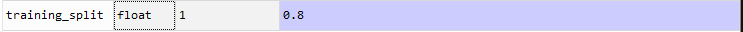
\includegraphics[width=0.5\textwidth]{figures/im/suara5.png}}
		\caption{Hasil Pemecahan Data Training dan Testing.}
		\label{suara5}
		\end{figure}

\item Praktekkan dan jelaskan masing-masing parameter dari fungsi Sequential(). \par
\lstinputlisting[firstline=106, lastline=111]{src/ron/Genre.py}
Sebuah model untuk menentukan aktivasi pada setiap neuron, di sini terdapat dense 100 merupakan 100 neurons pertama dari data training. Fungsi relu itu sendiri untuk melakukan aktivasi dari neuron-neuron atau inputan yang memiliki nilai maksimal. Sedangkan untuk dense 10 itu merupakan keluaran dari hasil neuron yang telah berhasil di aktivasi, untuk dense 10 ini di aktivasi dengan menggunakan softmax. Pada code tersebut tidak menampilkan keluran, hanya menampilkan code yang dijalankan seperti gambar \ref{suara6}
		\begin{figure}[!htbp]
		\centerline{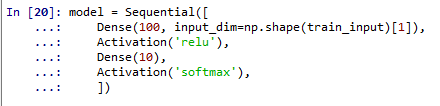
\includegraphics[width=0.5\textwidth]{figures/im/suara6.png}}
		\caption{Fungsi Sequential.}
		\label{suara6}
		\end{figure}

\item Praktekkan dan jelaskan masing-masing parameter dari fungsi compile(). \par
\lstinputlisting[firstline=113, lastline=116]{src/ron/Genre.py}
Hasil keluaran pada code tersebut seperti gambar \ref{suara7} menjelaskan bahwa dense pertama itu memiliki 100 neurons dengan parameter sekitar 2 juta lebih dengan aktviasi 100, jadi untuk setiap neurons memiliki masing-masing 1 aktivasi. Sama halnya seperti dense 2 memiliki jumlah neurons sebanyak 10 dengan parameter 1010 dan jumlah aktivasinya 10 untuk setiap neurons tersebut dan total parameternya sekitar 2.5 juta data yang akan dilatih pada mesin tersebut.
		\begin{figure}[!htbp]
		\centerline{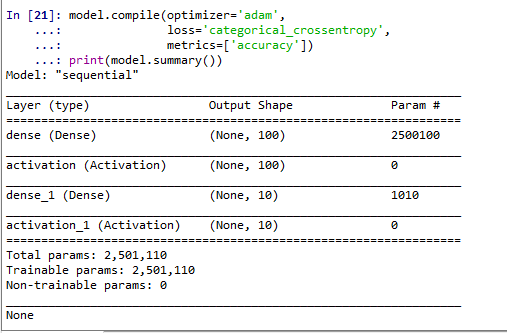
\includegraphics[width=0.5\textwidth]{figures/im/suara7.png}}
		\caption{Fungsi Compile.}
		\label{suara7}
		\end{figure}

\item Praktekkan dan jelaskan masing-masing parameter dari fungsi fit(). \par
\lstinputlisting[firstline=118, lastline=119]{src/ron/Genre.py}
Code tersebut untu melatih mesin dengan data training input dan training label. Epochs ini merupakan iterasi atau pengulangan berapa kali data tersebut akan dilakukan. Batch\_size ini adalah jumlah file yang akan dilakukan pelatihan pada setiap 1 kali pengulangan. Sedangkan validation\_split itu untuk menentukan presentase dari cross validation atau k-fold sebanyak 20\% dari masing-masing data pengulangan. Hasilnya bisa dilihat pada gambar \ref{suara8}
		\begin{figure}[!htbp]
		\centerline{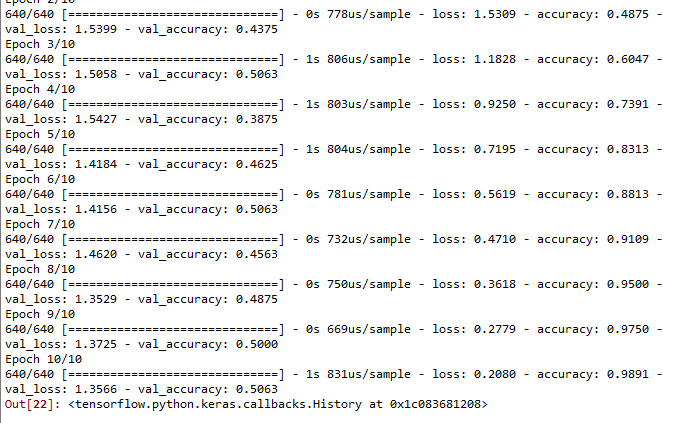
\includegraphics[width=0.5\textwidth]{figures/im/suara8.png}}
		\caption{Fungsi Fit.}
		\label{suara8}
		\end{figure}

\item Praktekkan dan jelaskan masing-masing parameter dari fungsi evaluate(). \par
\lstinputlisting[firstline=121, lastline=124]{src/ron/Genre.py}
Fungsi dari evaluate ini untuk mengevaluasi dari data testing dari masing-masing file. Di sini terdapat prediksi yang loss, maksudnya data yang diprediksi mesin itu salah, sedangkan untuk akurasi keseluruhannya sekitar 55\%. Untuk hasilnya bisa dilihat pada gambar \ref{suara9}
		\begin{figure}[!htbp]
		\centerline{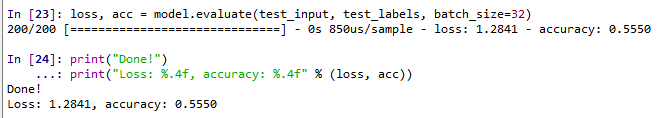
\includegraphics[width=0.5\textwidth]{figures/im/suara9.png}}
		\caption{Fungsi Evaluate.}
		\label{suara9}
		\end{figure}

\item Praktekkan dan jelaskan masing-masing parameter dari fungsi predict(). \par
\lstinputlisting[firstline=127, lastline=127]{src/ron/Genre.py}
Code tersebut akan melakukan testing satu data lagu dan hasilnya seperti gambar \ref{suara10}. Gambar tersebut menjelaskan file yang di jalankan tersebut termasuk ke dalam genre apa, hasilnya bisa dilihat pada gambar tersebut presentase yang paling besar yakni genre rock. Maka lagu tersebut termasuk ke dalam genre rock dengan perbandingan presentase hasil prediksi.
		\begin{figure}[!htbp]
		\centerline{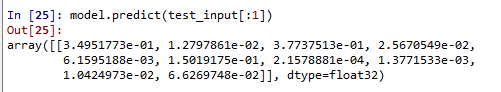
\includegraphics[width=0.5\textwidth]{figures/im/suara10.png}}
		\caption{Fungsi Predict.}
		\label{suara10}
		\end{figure}
\end{enumerate}

\subsection{Penanganan Error / Imron Sumadireja / 1164076}
\begin{enumerate}
\item Screenshot error \ref{nn1}
		\begin{figure}[!htbp]
		\centerline{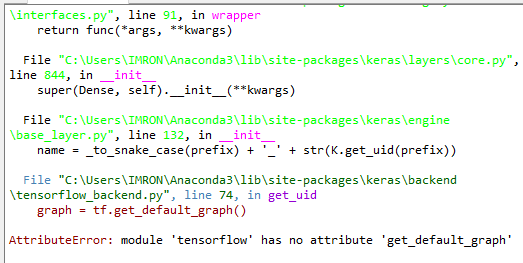
\includegraphics[width=0.5\textwidth]{figures/im/errorNN1.png}}
		\caption{Error TensorFlow.}
		\label{nn1}
		\end{figure}
\item Tuliskan kode error dan jenis errornya
\lstinputlisting[firstline=106, lastline=111]{src/ron/Genre.py}
Jenis errornya tidak terdapatnya atribut get default graph pada module tensorflow

\item Solusi pemecahan masalah error
\lstinputlisting[firstline=7, lastline=9]{src/ron/Genre.py}
Dengan menambahkan tensorflow.python pada library keras. Sehingga saat melakukan running code tersebut tidak akan menemukan error kembali, karena atribut get default graphnya sudah terpanggil.
\end{enumerate}

\section{Yusniar Nur Syarif Sidiq / 1164089}
\subsection{Pemahaman Teori Yusniar Nur Syarif Sidiq / 1164089}
\begin{enumerate}

\item Jelaskan kenapa file suara harus di lakukan MFCC. dilengkapi dengan ilustrasi !
	\subitem MFCC (Mel Frequency Cepstrum Coefficients) merupakan metode untuk melakukan feature extraction, sebuah proses yang mengkonversikan signal suara menjadi beberapa parameter. Dimana dalam python MFCC digunakan untuk melakukan etraction suara menjadi bentuk vektor. Mengapa perlu dilakukan ?, dikarenakan mesin tidak dapat membaca data selain bilangan biner dan vektor, maka dari itu untuk mempermudah pembacaan data oleh mesi perlu dilakukannya MFCC. Disini saya akan memberikan ilustrasi sederhana dimana ada sebuah Mechine Learning yang ingin membaca data dalam bentuk gelombang suara. Mechine Learning tidak akan bisa membaca data tersebut, Mengapa ?, karena data tersebut masih berbentuk gelombang suara, untuk memahami Mechine Learning perlu data dalam bentuk vektor, maka gelombang suara tersebut akan diubah menjadi bentuk vektor.

\item Jelaskan konsep dasar neural network. Dilengkapi dengan ilustrasi atau gambar !
	\subitem Neural Network atau Jaringan Saraf dimana memiliki neuron dan pada tiap neuron akan saling terhubung pada lapisan - laposan berikutnya. Pada lapisan pertama dimana terjadinya proses menerima input sedangkan pada lapisan terakhir akan memberikan output. Neural Network akan mengadopsi mekanisme berpikir sebuah sistem atau aplikasi yang menyerupai otak manusia, baik dalam pemrosesan berbagai sinyal elemen yang diterima, toleransi kesalahan atau error, dan parallel processing. Dimana terdapat dua data apel dan jeruk, data tersebut akan diinputkan pada setiap layer. Data tersebut akan dilakukan proses hidden pada hidden layer. Data yang dinputkan tadi akan diubah kedalam bentuk binner, dan outputnya akan terjadi misalnya 01 itu adalah apel dan 10 itu adalah jeruk. Untuk contoh figure dapat dilihat pada figure \ref{YNC6-1}.

	\begin{figure}[!htbp]
		\centering{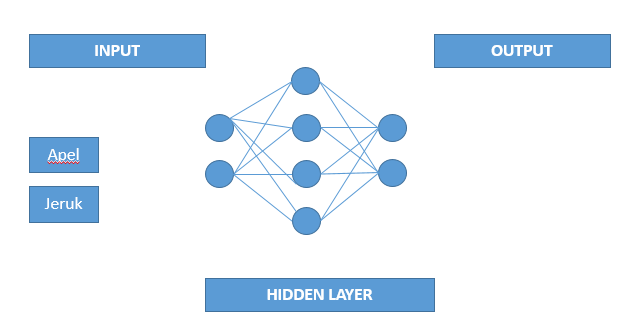
\includegraphics[scale=0.5]{figures/YN/Chapter6/Teori/YNC6-1.png}}
		\caption{Konsep Nural Network}
		\label{YNC6-1}
	\end{figure}

\item Jelaskan konsep pembobotan dalam neural network. Dilengkapi dengan ilustrasi atau gambar !
	\subitem Dimana Bobot akan mewakili koneksi antar unit. Apabila bobot dari node 1 ke node 2 memiliki nilai yang kebih besar, hal ini menandakan bahwa neuron 1 memiliki pengaruh yang lebih besar terhadap neuron 2. Apabila nilai bobot mendekati nol hal ini menandakan akan merubah input namun tidak mengubah output dan apabila nilai bobot negatif hal ini menandakan akan meningkatkan input namun mengurangi output yang artinya bobot akan menentukan seberapa besar pengaruh input terhadap output. Untuk ilustrasi figure dapat dilihat pada figure \ref{YNC6-2}.

	\begin{figure}[!htbp]
		\centering{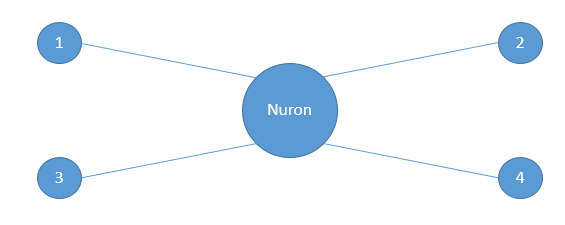
\includegraphics[scale=0.5]{figures/YN/Chapter6/Teori/YNC6-2.png}}
		\caption{Konsep Pembobotan}
		\label{YNC6-2}
	\end{figure}	

\item Jelaskan konsep fungsi aktivasi dalam neural network. Dilengkapi dengan ilustrasi atau gambar !
	\subitem Dimana fungsi aktivasi ini merupakan operasi dalam matematika yang digunakan pada sinyal output y. Fungsi ini sering digunakan untuk mengaktifkan atau menonaktifkan neuron. Dimana perilaku dari nural network ini ditentukan oleh bobot dan input-output fungsi aktivasi yang telah ditetapkan. Contohnya dimana jaringan lapisan tunggal akan menkonversi nilai input dari suatu variabel yang bernilai continue ke suatu nilai output biner yaitu angka 0 dan 1. Untuk contoh figure dapat dilihat pada pada figure \ref{YNC6-3}

	\begin{figure}[!htbp]
		\centering{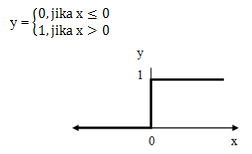
\includegraphics[scale=0.5]{figures/YN/Chapter6/Teori/YNC6-3.png}}
		\caption{Fungsi Aktivasi}
		\label{YNC6-3}
	\end{figure}	
	
\item Jelaskan cara membaca hasil plot dari MFCC. Dilengkapi dengan ilustrasi atau gambar !
	\subitem Perhatikan figure \ref{YNC6-4}, dimana terlihat bahwa warna biru merupakan suara terendah, mengapa ?, dikarenakan warna biru bernilai -300, sedangkan warna merah merupakah suara tertinggi dan bernilai 200. Jika diilustrasikan ada sebuah musik yang sedang dimainkan dan diperoleh datanya lalu diplot, maka akan terlihat seperti pada figure \ref{YNC6-4}

	\begin{figure}[!htbp]
		\centering{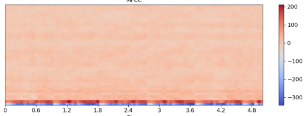
\includegraphics[scale=0.5]{figures/YN/Chapter6/Teori/YNC6-4.png}}
		\caption{Plot MFCC}
		\label{YNC6-4}
	\end{figure}	

\item Jelaskan apa itu one-hot encoding. Dilengkapi dengan ilustrasi kode dan atau gambar !
	\subitem One-hot encoding merupakan representasi variabel berkategorikan sebagai vektor biner yang artinya hanya akang 0 dan 1. Dimana mengharuskan nilai categorinya berbentuk biner dan setiap nilai integer akan dipresentasikan kedalam vektor biner. Contoh figure dapat dilihat pada figure \ref{YNC6-5}

	\begin{figure}[!htbp]
		\centering{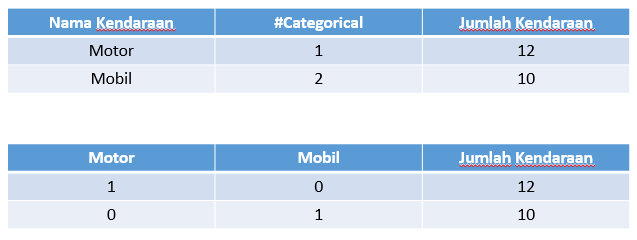
\includegraphics[scale=0.5]{figures/YN/Chapter6/Teori/YNC6-5.png}}
		\caption{One-Hot Encoding}
		\label{YNC6-5}
	\end{figure}	

\item Jelaskan apa fungsi dari np.unique dan to\_categorical dalam kode program . Dilengkapi dengan ilustrasi atau gambar !
	\subitem Fungsi dari np.unique yaitu sebagai indeks array input yang memberikan nilai unik, sebagai indeks array unik yang merekonstruksi array input, dan menghitung berapa kali setiap nilai unik muncul dalam array input. Contoh source code dalam pemrograman dapat dilihat pada figure \ref{YNC6-6}

	\begin{figure}[!htbp]
		\centering{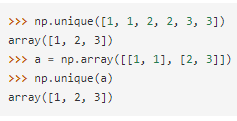
\includegraphics[scale=0.5]{figures/YN/Chapter6/Teori/YNC6-6.png}}
		\caption{np.unique}
		\label{YNC6-6}
	\end{figure}	

	\subitem Fungsi dari to\_categorical yaitu untuk mengubah vektor ke dalam matriks class biner. Contoh source code to\_categorical dapat dilihat pada figure \ref{YNC6-7}

	\begin{figure}[!htbp]
		\centering{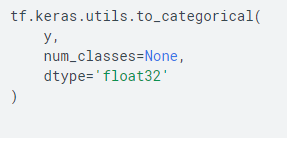
\includegraphics[scale=0.5]{figures/YN/Chapter6/Teori/YNC6-7.png}}
		\caption{categorical}
		\label{YNC6-7}
	\end{figure}	

\item Jelaskan apa fungsi dari Sequential dalam kode program. Dilengkapi dengan ilustrasi atau gambar !
	\subitem Dimana fungsi dari Sequential dalam source code program hanyalah sebagai tumpukan linear lapisan, dimana contih source code dalam program dapat dilihat pada figure \ref{YNC6-8}

	\begin{figure}[!htbp]
		\centering{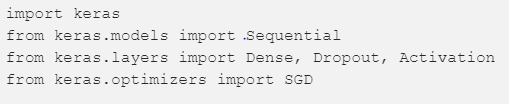
\includegraphics[scale=0.5]{figures/YN/Chapter6/Teori/YNC6-8.png}}
		\caption{Sequential}
		\label{YNC6-8}
	\end{figure}

\end{enumerate}

\subsection{Praktek Program / Yusniar Nur Syarif Sidiq / 1164089}
\begin{enumerate}

\item Jelaskan isi dari data GTZAN genre collection dan data dari freesound. Buat kode program untuk meload data tersebut untuk digunakan pada MFCC. Jelaskan arti dari setiap baris kode yang dibuat !
	\subitem Dimana data GTZAN merupakan dataset yang terdiri dari 10 genre lagu yang berbeda beda dan masing-masing genre memiliki 100 lagu. Jika kita ingin melakukanload data tersebut source code sederhananya dapat dilihat sebagai berikut,
	\lstinputlisting[firstline=134, lastline=135]{src/yns/GenreIdentifier.py}
Dimana source code tersebut akan melakukan load pada data yang ber genre blus dengan durasi selama 30 detik.

\item Jelaskan perbaris kode program dengan kata-kata dan dilengkapi ilustrasi gambar fungsi dari display\_mfcc() !
	\lstinputlisting[firstline=25, lastline=25]{src/yns/GenreIdentifier.py}
	\subitem Perhatikan figure \ref{YNC6-9}, dimana pada figure tersebut memiliki data hz dan time. Dalam figure tersebut memiliki warna yang berbeda. Pada warna biru, menunjukkan power berada di titik terendah sedangkan warna biru menunjukkan power berada di titik tertinggi.

	\begin{figure}[!htbp]
		\centering{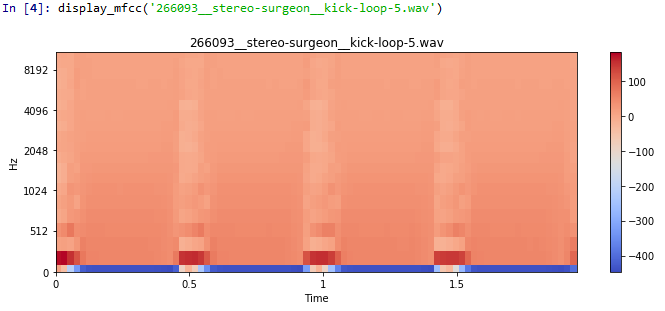
\includegraphics[scale=0.5]{figures/YN/Chapter6/Praktek/YNC6-9.png}}
		\caption{Output Pada Fungsi Display}
		\label{YNC6-9}
	\end{figure}

\item Jelaskan perbaris kode program dengan kata-kata dan dilengkapi ilustrasi gambar fungsi dari ectract\_features\_song(). Jelaskan juga mengapa yang diambil 25.000 baris pertama !
	\lstinputlisting[firstline=48, lastline=58]{src/yns/GenreIdentifier.py}
	\subitem Pada source code tersebut akan menghasilkan output seperti pada figure \ref{YNC6-10}, Mengapa kita cuman mengambil 25.000 data pertamanya saja ?, dikarenakan untuk meringankan kinerja laptop kita sehingga tidak memakan memory lebih besar, maka dari itu kita batasi data yang diambil hanya 25.000.

	\begin{figure}[!htbp]
		\centering{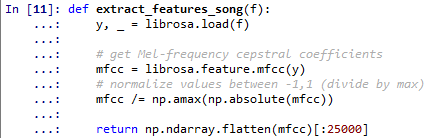
\includegraphics[scale=0.5]{figures/YN/Chapter6/Praktek/YNC6-10.png}}
		\caption{Output Instasiasi Pada Fungsi ectract\_features\_song()}
		\label{YNC6-10}
	\end{figure}

\item  Jelaskan perbaris kode program dengan kata-kata dan dilengkapi ilustrasi gambar fungsi dari generate\_feature\_and\_labels() !
	\lstinputlisting[firstline=62, lastline=79]{src/yns/GenreIdentifier.py}
	\subitem Dimana source code tersebut akan melakukan fungsi pada source code sebelumnya. Data generes merupakan dataset yang telah kita download. Lalu kita akan melakukan looping atau pengulangan untuk file yang berekstensi .au dan akan melakuan ekstrak pada folder genres. File yang diekskrak akan dibentuk menjadi vektor dan dimasukkan kedalam fitur. Append akan melakukan penumpukan file yang sudah dilaukan vektorisasi.

\item Jelaskan dengan kata dan praktek kenapa penggunaan fungsi generat\_features\_and\_labels() sangat lama ketika meload dataset genre !
	\lstinputlisting[firstline=83, lastline=83]{src/yns/GenreIdentifier.py}
	\subitem Hal ini dikarenakan mesin akan melakukan vektorisasi kepada file yang berada dalam folder genres. Dalam folder genres terdapat 10 folder dan masing-masing folder terdapat 100 data dan data tersebut akan dilakukan vektorisasi atau melakukan ekstrasi menggunakan fitur mfcc. Maka dari itu fungsi tersebut akan memakan waktu yang cukup lama. Hasil output dari source code nya dapat dilihat pada figure \ref{YNC6-11}

	\begin{figure}[!htbp]
		\centering{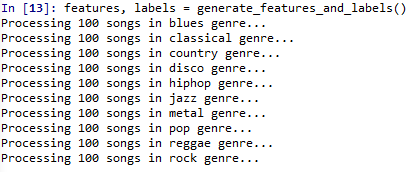
\includegraphics[scale=0.5]{figures/YN/Chapter6/Praktek/YNC6-11.png}}
		\caption{Output Pada Source Code generate\_feature\_and\_labels()}
		\label{YNC6-11}
	\end{figure} 

\item dilakukan pemisahan data training dan data set sebesar 80\% ? Praktekkan dengan kode dan tunjukkan keluarannya dari komputer sendiri dan artikan maksud setiap luaran yang didapatkan !
	\lstinputlisting[firstline=88, lastline=88]{src/yns/GenreIdentifier.py}
	\subitem Supaya mesin akan belajar tentang data-data testing atau data baru sehingga pada saat dilakukan training dan di prediksi dapat menunjukkan presentase yang baik. Hasil dari source codenya dapat dilihat pada figure \ref{YNC6-12}

	\begin{figure}[!htbp]
		\centering{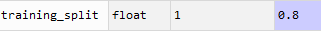
\includegraphics[scale=0.5]{figures/YN/Chapter6/Praktek/YNC6-12.png}}
		\caption{Pemisahan Data Training Dan Testing}
		\label{YNC6-12}
	\end{figure} 

\item Praktekkan dan jelaskan masing-masing parameter dari fungsi Sequential() !
	\lstinputlisting[firstline=110, lastline=115]{src/yns/GenreIdentifier.py}
	\subitem Dimana model tersebut akan menentukan aktivasi dalam setiap neuron. Dimana pada kasus kali ini terdaoat 100 neurons pada data training. Pada source code tercantum Activation relu yang dimana fungsinya akan melakukan aktivasi terhadap neuron yang memiliki nilai max. Hasil penguluaran akan ditunjukan oleh dense. Dense akan dilakukan aktivasi menggunakan softmax. Hasil source code akan menunjukkan proses intasiasi yang ditunjukkan pada figure \ref{YNC6-13}

	\begin{figure}[!htbp]
		\centering{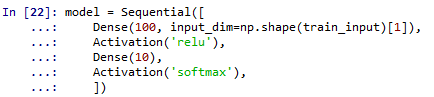
\includegraphics[scale=0.5]{figures/YN/Chapter6/Praktek/YNC6-13.png}}
		\caption{Sequential}
		\label{YNC6-13}
	\end{figure} 	

\item Praktekkan dan jelaskan masing-masing parameter dari fungsi compile() !
	\lstinputlisting[firstline=117, lastline=120]{src/yns/GenreIdentifier.py}
	\subitem Dimana source code tersebut akan menampilkan data dense pertama berjumlah 100 neurons dan memiliki parameters sebanyak 2500100 dan aktivasi 100 yang dimana setiap 1 neuraons memiliki 1 aktivasi. Untuk dense 2 sama saja seperti dense 1 hanya saja datanya yang berbeda. Hasil output yang diberikan akan terlihat seperti figure \ref{YNC6-14}

	\begin{figure}[!htbp]
		\centering{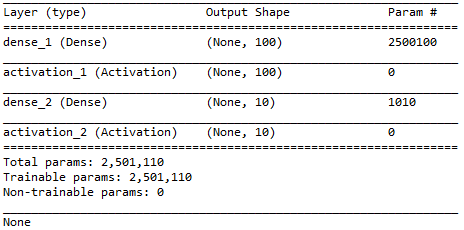
\includegraphics[scale=0.5]{figures/YN/Chapter6/Praktek/YNC6-14.png}}
		\caption{Fungsi Compile}
		\label{YNC6-14}
	\end{figure} 	

\item Praktekkan dan jelaskan masing-masing parameter dari fungsi fit() !
	\lstinputlisting[firstline=121, lastline=125]{src/yns/GenreIdentifier.py}
	\subitem Dimana source code akan melakukan training pada mesin dengan data training input dan data training label. Terdapat epochs yang menunjukan berapa kali data tersebut akan diulang. Lalu ada batch\_size yang dimana artinya menunjukkan jumlah file yang akan dilakukan training dalam setiap satu kali pengulangan. Lalu validation\_split akan menunjukkan score dari validasi silang sebanyak 0.2 atau dalam presentase yaitu 20\% untuk setiap data pengulangan. Hasil dari output source code dapat dilihat pada figure \ref{YNC6-15}

	\begin{figure}[!htbp]
		\centering{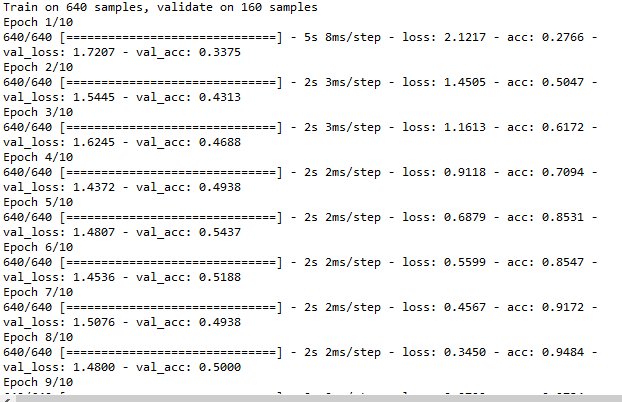
\includegraphics[scale=0.5]{figures/YN/Chapter6/Praktek/YNC6-15.png}}
		\caption{Fungsi Fit}
		\label{YNC6-15}
	\end{figure} 	

\item Praktekkan dan jelaskan masing-masing parameter dari fungsi evaluate() !
	\lstinputlisting[firstline=125, lastline=128]{src/yns/GenreIdentifier.py}
	\subitem Diamana fungsi ini akan mengevaluasi data testing pada setiap file. Data loss menunjukkan hasil prediksi mesin yang salah dan akurasi yang dihasilkan yaitu 0.6100 atau dalam presentase yaitu 61\%. Hasil dari source code dapat dilihat pada figure \ref{YNC6-16}

	\begin{figure}[!htbp]
		\centering{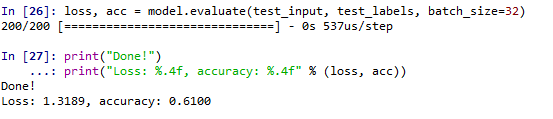
\includegraphics[scale=0.5]{figures/YN/Chapter6/Praktek/YNC6-16.png}}
		\caption{Fungsi Evaluate}
		\label{YNC6-16}
	\end{figure} 	

\item Praktekkan dan jelaskan masing-masing parameter dari fungsi predict() !
	\lstinputlisting[firstline=131, lastline=131]{src/yns/GenreIdentifier.py}
	\subitem Dimana pada source code tersebut akan melakukan prediksi pada data testing dan hanya satu data testing sehingga dapat dijelaskan data testing tersebut termasuk kedalam genre yang mana. Hasilnya akan ditampilkan kedalam bentuk ndarray. Output yang diberikan dapat dilihat pada figure \ref{YNC6-17}

	\begin{figure}[!htbp]
		\centering{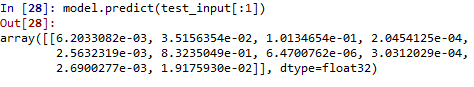
\includegraphics[scale=0.5]{figures/YN/Chapter6/Praktek/YNC6-17.png}}
		\caption{Fungsi Predict}
		\label{YNC6-17}
	\end{figure} 	

\end{enumerate}

\subsection{Penangan Error / Yusniar Nur Syarif Sidiq / 1164089}
\begin{enumerate}

\item Screenshoot Error yang di dapat figure \ref{YNC6-18}. 
	
	\begin{figure}[!htbp]
		\centering{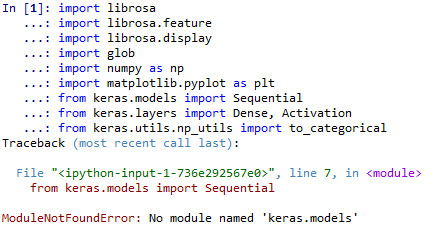
\includegraphics[scale=0.5]{figures/YN/Chapter6/Praktek/YNC6-18.png}}
		\caption{Fungsi Evaluate}
		\label{YNC6-18}
	\end{figure} 

\item Tuliskan kode error dan jenis errornya dan bagaimana cara menanganinya.
		\lstinputlisting[firstline=139, lastline=148]{src/yns/GenreIdentifier.py}


\end{enumerate}